\documentclass{beamer}
\usepackage{ulem}
\usepackage{tikz}
\usepackage{booktabs}
\usepackage{graphicx,threeparttable,caption}
\usetikzlibrary{shapes,snakes}
\usepackage[beamer,customcolors]{hf-tikz}
\usepackage{nicematrix}
\usepackage{xcolor}
\usepackage{makecell}
\usepackage{array}
\usepackage{csquotes}
\usepackage{csquotes}
\usepackage{minted}
\captionsetup{labelformat=empty,labelsep=none}

\graphicspath{ {./png/} }

\usetikzlibrary{
    arrows,
    arrows.meta,
    shapes,
    positioning,
    shadows,
    trees,
    calc
}

\tikzset{%
    >={Latex[width=2mm,length=2mm]},
    % Specifications for style of nodes:
    plain/.style = {},
    base/.style = {
        plain,
        rectangle, rounded corners, draw=black,
        minimum width=1cm, minimum height=1cm,
        text centered, font=\sffamily\tiny\bfseries,
        fill=white, align=center
    },
    app/.style = {base, ellipse},
    data/.style = {base, fill=gray!30},
    action/.style = {base, circle, fill=red!30},
    note/.style = {app, fill=yellow},
    hl/.style={
    set fill color=red!80!black!40,
    set border color=red!80!black
    }
}


\AtBeginSection[]{
  \begin{frame}
  \vfill
  \centering
  \begin{beamercolorbox}[sep=8pt,center,shadow=true,rounded=true]{title}
    \usebeamerfont{title}\insertsectionhead\par%
  \end{beamercolorbox}
  \vfill
  \end{frame}
}
\setbeamercolor{alerted text}{fg=red}
%\usecolortheme[orchid]{structure}
\usetheme[hideothersubsections]{PaloAlto}
\makeatletter
\patchcmd{\csq@bquote@i}{{#6}}{{\emph{#6}}}{}{}
\makeatother
%\usecolortheme{orchid}
%\usefonttheme{professionalfonts}
\newcommand{\soutthick}[1]{%
   \textcolor{red}{
   \renewcommand{\ULthickness}{1pt}%
      \sout{#1}%
   \renewcommand{\ULthickness}{.4pt}% Resetting to ulem default
   }
}
\newcommand{\centered}[1]{\begin{tabular}{l} #1 \end{tabular}}
\setbeamertemplate{section in toc}[square]
\setbeamertemplate{subsection in toc}[square]
\setbeamertemplate{section in sidebar}[shaded]
\setbeamertemplate{items}[square]
\setbeamercovered{transparent} 

\title[]{Introduction to Computational Social Science}
\subtitle{Presentations}
\author[]{Mikołaj Biesaga\\ \small{\color{blue}{\href{mailto:m.biesaga@uw.edu.pl}{m.biesaga@uw.edu.pl}}}}
\institute{
\includegraphics[width = 4 cm]{uw.png}}
\date{April 1, 2025}
\begin{document}
\begin{frame}
   \titlepage
\end{frame}

\part{Presentations}
\section[Presentations]{Presentations}
\begin{frame}{Structure of the presentation}
    \begin{itemize}
     \item \textbf{Introduction and problem statement.} This section should
     explain what is the project about in general and why the given problem
     matters. The significance of the problem may be justified both in terms of
     its theoretical/scientific or societal/business relevance.
     \item \textbf{Research question.} What is the specific research question
     the paper tries to answer? It can be either formulated as a
     strict hypothesis or as an exploratory question.
     \item \textbf{Research methods.} This section should discuss, at a general
     level, what data was collected and how.     
    \end{itemize}
\end{frame}
    
\begin{frame}{Structure of the presentation}
    \begin{itemize}
     \item \textbf{Analytic methods.} What analytic methods were applied to
     answer the research question? This may include some methods
     that we discussed in the class (i.e. sentiment analysis or some other
     natural language processing methods), but not necessarily.
     \item \textbf{Results.} What were the main results? You don't have to
     go too much into detail, i.e., report statistical test results. Explain
     what was tested which hypotheses were rejected and for which there was no proof to reject them.    
     \item \textbf{Conclusions.} Discuss the results within the broader context of
     the literature (you can either do it based on the paper or you can interpret
     the results based on your knowledge). What is the take-home message?
    \end{itemize}
\end{frame}
    
\section[Things to remember]{Things to remember}
\begin{frame}{Things to remember}
    \begin{itemize}
     \item Half an hour is less time than you think. \alert{Make up to 20 slides}.
     \item Begin by explaining the structure of the presentation.
     \item \alert{Use as many pictures/schemes as possible}.
     \item Don't use fancy transitions unless there is a good reason for that.
     \item Use colors wisely.
     \item Don't put too much bibliography in the slides. Unless it is something crucial.
     \item Rehearse your presentation before you give it.
    \end{itemize}
\end{frame}
    
\section[Formal requirements]{Formal requirements}
\begin{frame}
        \frametitle{Formal requirements}
        \only<1>{
            \begin{itemize}
            \item The presentation must be based on a \alert{scientific research paper}.
            \item The paper should use computational methods.
            \item The presentation should not exceed \alert{30 minutes}.
            \item People asking questions should prepare at least two questions based on 
            the paper. 
            \end{itemize}
        }
        \only<2>{
            \begin{block}{}
                Last but not least, the presentation must look aesthetically. Please, spend
                some time on formatting, checking spelling and grammar.
            \end{block}
        }
\end{frame}
\part{Smart Cities}
\section[Introduction]{Introduction}
\begin{frame}
    \frametitle{Introduction}
    \only<1-4>{
        \begin{itemize}
            \item \alert<1>{The smart-city discourse is presently in flux}, engaged
            in intensive boundary-work and evidently struggling to gain wider
            support on several fronts (Joss et al., 2019).
            \item The smart-city transitions often focus on creating the 
            narrative of \alert<2>{vaguely defined benefits of quick fixes to the
            existing issues} (Jir{\'o}n et al. 2021).
            \item \alert<3>{Threats resulting from the commodification and
            commercialisation of data by Big Tech}, which is further facilitated
            by smart-city technologies (Zuboff, 2019).
            \item The use of sensors and ICT tools in effort to "flatten the
            curve". The increase of smart city techologies implementation as a
            \alert<4>{response to the COVID-19 pandemic}.
        \end{itemize}
    }
    \only<5>{
        \framesubtitle{Motivation}
        \begin{block}{}
            We wanted to observe whether the \alert{COVID-19 pandemic changed}
            the narrative on the transition of European cities into smart cities
            and consequently \alert{accelerated the implementation of smart city
            technologies}. We expected that the intensity of the changes shifted
            the existing narrative towards threats that excessive data
            collection on citizens may pose.
        \end{block}
    }
\end{frame}
\section{Method}
\begin{frame}
   \frametitle{Method}
   \framesubtitle{Analysis Strategy}
   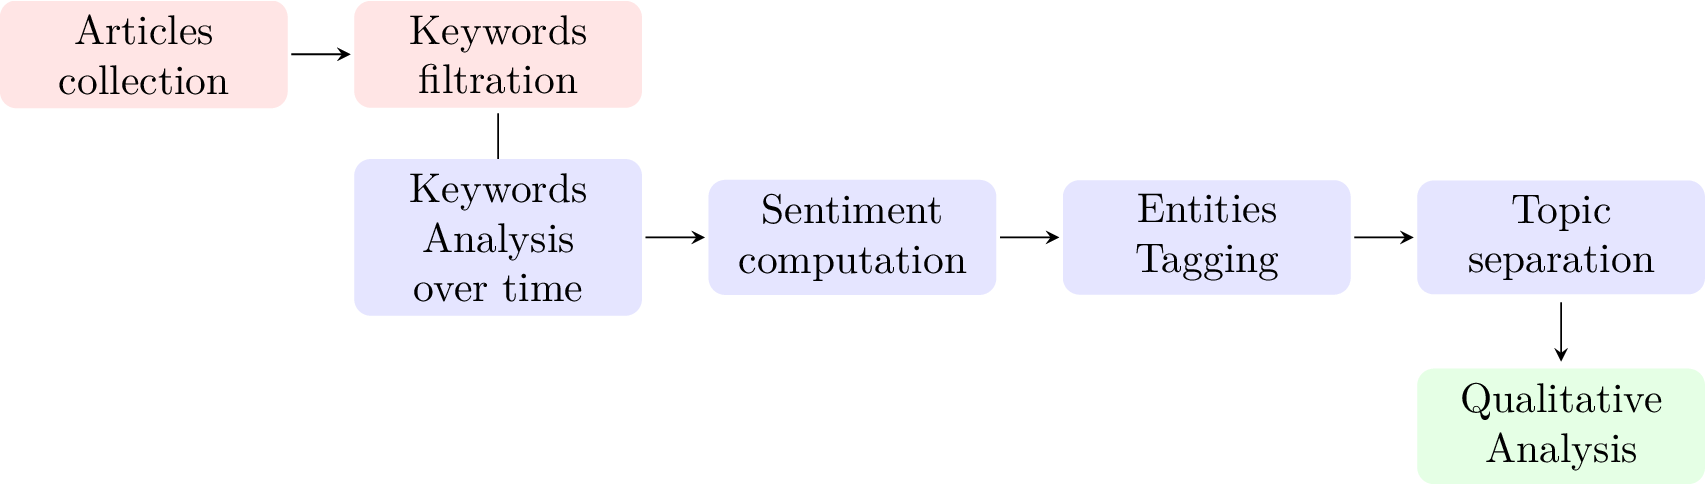
\includegraphics[width = \textwidth]{scheme.png}
\end{frame}
\begin{frame}[t]
   \frametitle{Method}
   \only<1-2>{
      \framesubtitle{Articles collection \& Keywords filtration}
      %\setbeamercolor{block body}{bg=red!10,fg=black}
      \begin{enumerate}
         \item<1-> Sources selection
         %\item<2-> Facebook posts collection
         \item<2> Articles collection
      \end{enumerate}
      \only<1>{
         \begin{block}
            \centering
            \scriptsize
            \setcellgapes{4pt}\makegapedcells
            \begin{tabular}{|p{.35\textwidth}|>{\centering}p{.27\textwidth}|>{\centering\arraybackslash}p{.23\textwidth}|}
                \hline
                \bfseries{Source name}& \bfseries{Facebook Followers} & \bfseries{Facebook Likes} \\
                \hline
                \hline
                POLITICO Europe & $164\ 065$ & $156\ 291$ \\
                \hline
                Euronews English & $2\ 182\ 331$ & $2\ 107\ 895$ \\
                \hline
                EUobserver & $139\ 582$ & $139\ 194$ \\
                \hline
                EURACTIV & $45\ 453$ & $42\ 790$ \\
                \hline
                The Parliament Magazine & $5\ 222$ & $4\ 850$ \\
                \hline
            \end{tabular}
      \end{block}
      }
%      \only<2>{
%         \begin{figure}
%            \centering
%            
\includegraphics{sotrender_black.png}
%         \end{figure}
%      }
      \only<2>{
         \begin{block}
            \centering
            \scriptsize
            \setcellgapes{4pt}\makegapedcells
            \begin{tabular}{|p{.35\textwidth}|>{\centering}p{.17\textwidth}|>{\centering}p{.17\textwidth}|>{\centering\arraybackslash}p{.13\textwidth}|}
                \hline
                \bfseries{Source name}& \bfseries{Complete corpus} & \bfseries{Reduced corpus} & \bfseries{Final corpus} \\
                \hline
                \hline
                POLITICO Europe & $12\ 660$ & $161$ & $48$\\
                \hline
                Euronews English & $35\ 172$ & $205$ & $43$\\
                \hline
                EUobserver & $10\ 924$ & $62$ & $22$\\
                \hline
                EURACTIV & $9\ 745$ & $156$ & $48$\\
                \hline
                The Parliament Magazine & $1\ 656$ & $41$ & $23$\\
                \hline
            \end{tabular}
      \end{block}
      }
   }
   \only<3>{
      \framesubtitle{Keywords Analysis over time}
      \begin{center}
         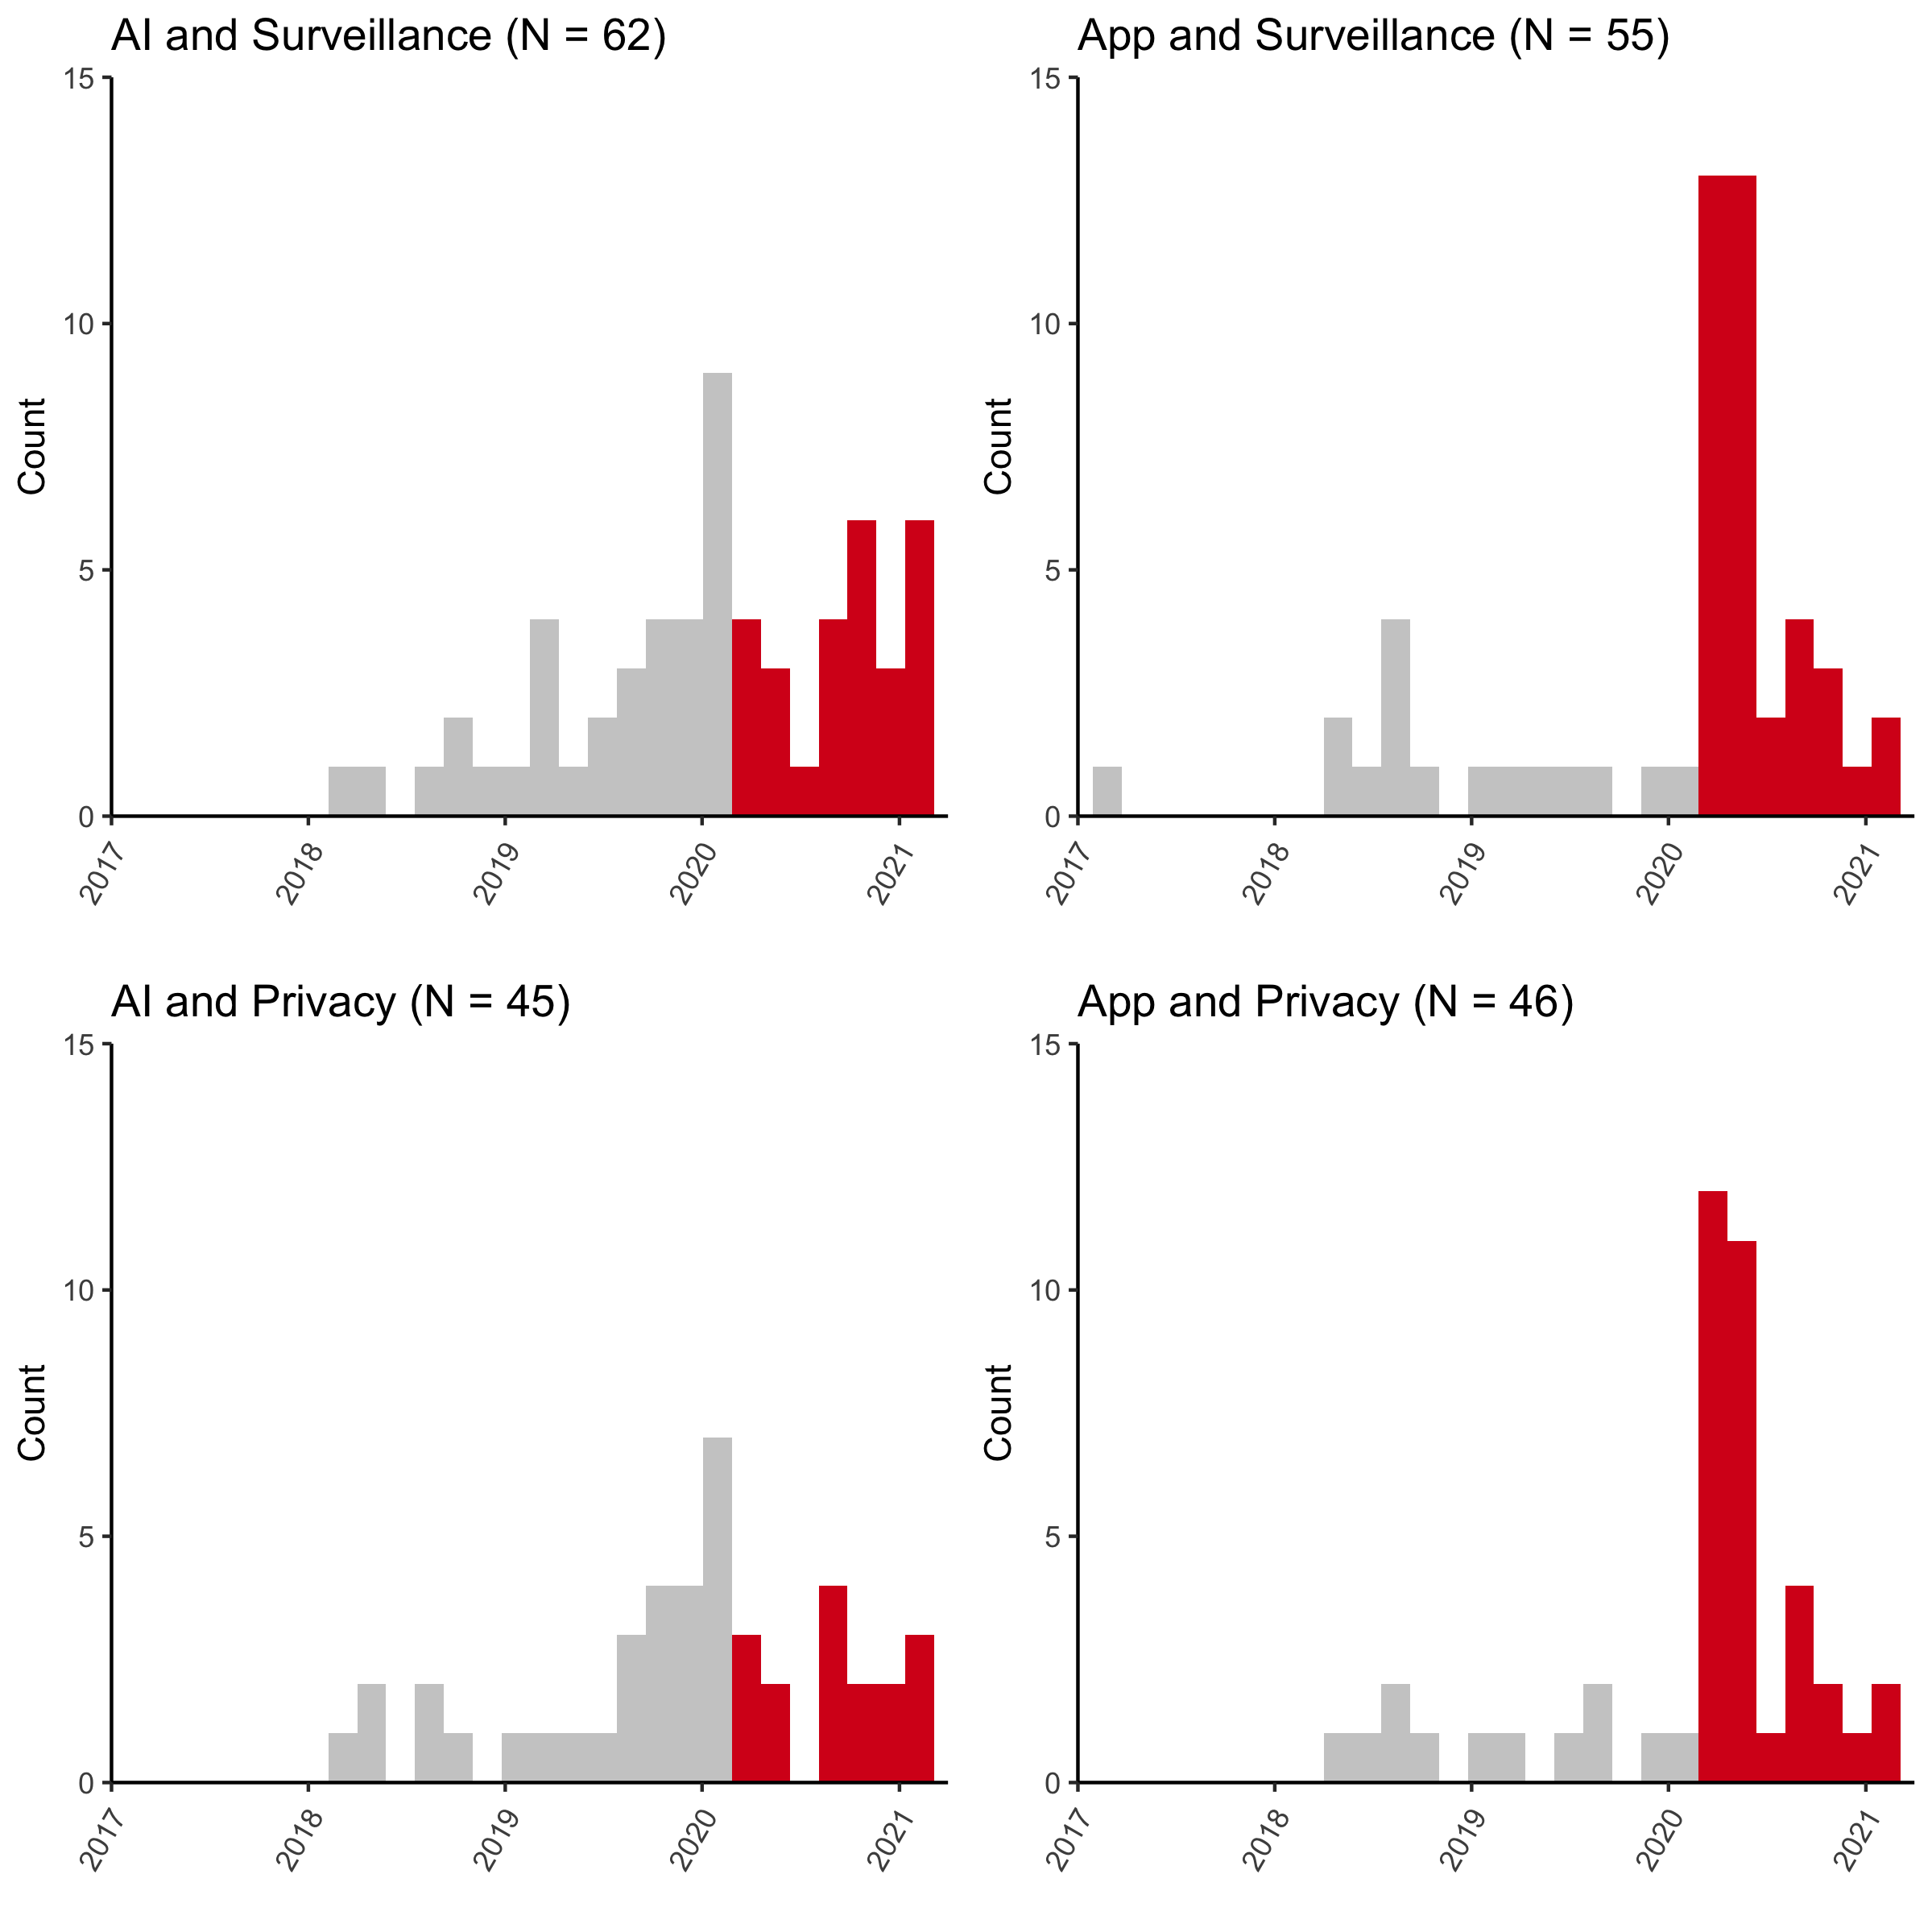
\includegraphics[width = .57\textwidth]{panel_plot.png}
      \end{center}
   }
   \only<4-7>{
      \framesubtitle{Sentiment Computation \& Entities Tagging \& Topic separation}
      \begin{itemize}
         \item<4-> Automatic Sentiment Computation\only<4>{\footnote[1]{Hutto C., Gilbert, E. (2014). Vader: A parsimonious rule-based model for sentiment analysis of social media text. \textit{Proceedings of the International AAAI Conference on Web and Social Media}, 8(1).}}
         \item<5-> Entities Tagging\only<5>{\footnote[2]{Honnibal M., Montani, I., Van Landeghem, S. (2020) spaCy: Industrial-strength Natural Language Processing in Python. Software.}}
         \item<6-> Topic Separation -- Latent Dirichlet Allocation\only<6>{\footnote[3]{Blei, D.M., Ng, A.Y., Jordan M.I. (2003). Latent dirchlet allocation. \textit{Journal of machine Learning research}, 3:993--1022.}}
      \end{itemize}
%      \only<4>{
%         \begin{equation*}
%            Sentiment = compuond \times (1 - Neutral)
%         \end{equation*}
%      }
      \only<5>{
         \centering
         
\includegraphics[width = .4\textwidth]{spacy.png}
      }
      \only<6>{
         \begin{block}
            \centering
            \scriptsize
            \centering
            \setcellgapes{2pt}\makegapedcells
            \begin{tabular}{|p{.2\textwidth}|>{\centering\arraybackslash}p{.30\textwidth}|}
                \hline
                \bfseries{Topic} & \bfseries{Number of Articles} \\
                \hline
                \hline
                Topic 1 & $82$ \\
                \hline
                Topic 2 & $13$ \\
                \hline
                Topic 3 & $38$ \\
                \hline
                Topic 4 & $4$ \\
                \hline
                Topic 5 & $28$ \\
                \hline
                Topic 6 & $5$ \\
                \hline
                Topic 7 & $14$ \\
                \hline
            \end{tabular}
         \end{block} 
      }
      \only<7>{
         \begin{block}
            \centering
            \scriptsize
            \centering
            \setcellgapes{2pt}\makegapedcells
            \begin{tabular}{|p{.2\textwidth}|>{\centering\arraybackslash}p{.30\textwidth}|}
                \hline
                \bfseries{Topic} & \bfseries{Number of Articles} \\
                \hline
                \hline
                Topic 1 & $82$ \\
                \hline
                Topic 2 & $13$ \\
                \hline
                Topic 3 & $38$ \\
                \hline
                \soutthick{\textcolor{black}{Topic 5}} Topic 4 & $28$ \\
                \hline
            \end{tabular}
         \end{block} 
      }
   }
\end{frame}
\section{Quantitative Analysis}
\begin{frame}
   \frametitle{Quantitative Analysis}
   \setbeamertemplate{caption}{\raggedright\insertcaption\par}
   \settowidth{\leftmargini}{\usebeamertemplate{itemize item}}
   \addtolength{\leftmargini}{\labelsep}
   \only<1>{
      \framesubtitle{Topic 1: Artificial Intelligence and Facial Recognition.}
      \only<1>{
         \begin{block}
            \centering
            \scriptsize
            \centering
            \setcellgapes{2pt}\makegapedcells
            \begin{tabular}{|>{\centering\arraybackslash}p{.25\textwidth}|>{\centering\arraybackslash}p{.22\textwidth}|>{\centering\arraybackslash}p{.30\textwidth}|}
                \hline
                \bfseries{Qualitative Analysis Summary} & \bfseries{Surveillance and Privacy} & \bfseries{Actors} \\
                \hline
                \hline
                \begin{itemize}\item FR is a threat to privacy. \item AI bias is a threat to equality and justice. \item FR systems do not seem to be as effective in finding criminals as the police claims. \end{itemize}& \begin{itemize} \item \textbf{Surveillance} (0.8) \item \textbf{Privacy} (0.6) \end{itemize} & \begin{itemize} \item \textbf{Main actors}: EU (0.7), EC (0.5), China (0.4), Police (0.4), Facebook (0.3), France (0.3), Germany (0.3) and USA (0.3) \item \textbf{Secondary actors}: Amazon (0.2), Apple (0.1), Huawei (0.1) and Microsoft (0.1) \end{itemize} \\
                \hline
            \end{tabular}
         \end{block} 
      }
      %\includegraphics<2>[width = \textwidth]{topic-0-si-3-1.png}
   }
   \only<2>{
      \framesubtitle{Topic 2: Smart technologies and climate emergency.}
      \only<2>{
         \begin{block}
            \centering
            \scriptsize
            \centering
            \setcellgapes{2pt}\makegapedcells
            \begin{tabular}{|>{\centering\arraybackslash}p{.25\textwidth}|>{\centering\arraybackslash}p{.22\textwidth}|>{\centering\arraybackslash}p{.30\textwidth}|}
                \hline
                \bfseries{Qualitative Analysis Summary} & \bfseries{Surveillance and Privacy} & \bfseries{Actors} \\
                \hline
                \hline
                \begin{itemize}\item Smart technologies as a way forward in building climate neutrality. \item Chance for closing gaps. \item The threats related to recycling of technological waste and the heating effect of server farms. \end{itemize}& \begin{itemize} \item \textbf{Surveillance} (0.1) \item \textbf{Privacy} (0.1) \end{itemize} & \begin{itemize} \item \textbf{Main actors}: EU (0.7) and EC (0.4) \item \textbf{Secondary actors}: China (0.2), Germany (0.1), Sweden (0.1) and USA (0.1) \end{itemize} \\
                \hline
            \end{tabular}
         \end{block} 
      }
      %\includegraphics<4>[width = \textwidth]{topic-1-si-3-1.png}
   }
   \only<3>{
      \framesubtitle{Topic 3: Technology to fight the COVID-19 pandemic.}
%      \only<5>{
%         \begin{figure}
%            \includegraphics[width = \textwidth]{topic_03.png}
%            \caption{\alert{The left panel} shows the most probable words while \alert{the right panel} depicts probablity of the words that are unique only for the topic.}
%         \end{figure}
%      }
      \only<3>{
         \begin{block}
            \centering
            \scriptsize
            \centering
            \setcellgapes{2pt}\makegapedcells
            \begin{tabular}{|>{\centering\arraybackslash}p{.25\textwidth}|>{\centering\arraybackslash}p{.22\textwidth}|>{\centering\arraybackslash}p{.30\textwidth}|}
                \hline
                \bfseries{Qualitative Analysis Summary} & \bfseries{Surveillance and Privacy} & \bfseries{Actors} \\
                \hline
                \hline
                \begin{itemize}\item Technologies help Europe recover from the crippling effects of the COVID-19 crisis. \item Tracking apps as 'necessary evil'. \item A close collaboration between public sector and private corporations is a potential threat to privacy. \end{itemize}& \begin{itemize} \item \textbf{Surveillance} (0.7) \item \textbf{Privacy} (0.8) \end{itemize} & \begin{itemize} \item \textbf{Main actors}: EU (0.5), France (0.5), Germany (0.5), EC (0.4), Google (0.4), Apple (0.3), Poland (0.3) and UK (0.3) \item \textbf{Secondary actors}: China (0.2) and Facebook (0.1) \end{itemize} \\
                \hline
            \end{tabular}
         \end{block} 
      }
      %\includegraphics<6>[width = \textwidth]{topic-2-si-3-1.png}
   }
   \only<4>{
      \framesubtitle{Topic 4: For digitalization of Europe.}
      \only<4>{
         \begin{block}
            \centering
            \scriptsize
            \centering
            \setcellgapes{2pt}\makegapedcells
            \begin{tabular}{|>{\centering\arraybackslash}p{.25\textwidth}|>{\centering\arraybackslash}p{.22\textwidth}|>{\centering\arraybackslash}p{.30\textwidth}|}
                \hline
                \bfseries{Qualitative Analysis Summary} & \bfseries{Surveillance and Privacy} & \bfseries{Actors} \\
                \hline
                \hline
                \begin{itemize}\item 5G as a tool for developing the EU digital market. \item Slow implementation of EU 5G infrastructure risks the dominance of non-European suppliers. \item Open debate on 5G's benefits and threats is needed in the EU. \end{itemize}& \begin{itemize} \item \textbf{Surveillance} (0.2) \item \textbf{Privacy} (0.2) \end{itemize} & \begin{itemize} \item \textbf{Main actors}: EU (0.7) and EC (0.5) \item \textbf{Secondary actors}: Amazon (0.2), Facebook (0.2), Google (0.1) and Huawei (0.1) \end{itemize} \\
                \hline
            \end{tabular}
         \end{block} 
      }
      %\includegraphics<8>[width = \textwidth]{topic-4-si-3-1.png}
   }
\end{frame}
\section{Qualitative Analysis}
\begin{frame}
   \frametitle{Qualitative Analysis}
   %% \only<1>{
   %%    \framesubtitle{Perceived Sentiment Analysis}
   %%    \centering
   %%    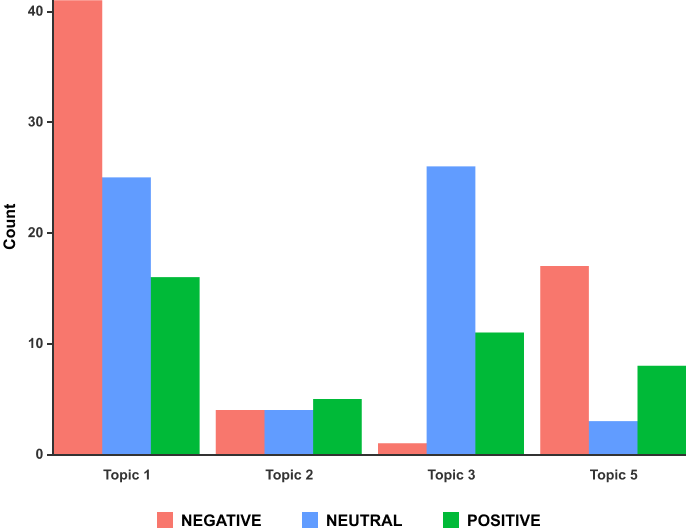
\includegraphics[width = .9\textwidth]{plot_sent.png}
   %% }
   %% \only<1-3>{
   %%    \framesubtitle{Qualitative analysis of topics}
   %%    \begin{itemize}
   %%       \item<1-> Pandemic as a fast-tracking factor in technological development
   %%       \item<2-> Privacy concerns
   %%       \item<3> Trade-off between health and privacy
   %%    \end{itemize}
   %%       \only<1>{\begin{block}{}
   %%          \blockquote[EUobserver, 2020-04-14]{%
   %%             \small The response of EU countries to the coronavirus outbreak has prompted unprecedented levels of surveillance, data expoitation, and misinformation. Data collection can be essentail to understand and respond to the COVID-19 emergency, but creating such digital surveillance risks failure and adverse side-effect.%
   %%          }
   %%       \end{block}
   %%       }
   %%       \only<2>{\begin{block}{}
   %%          \blockquote[POLITICO Europe, 2020-04-19]{%
   %%             \small And almost 40 governments worldwide have rolled out -- or are about to -- their own coronavirus apps for everything from informing people if they've been in contact with anyone infected with COVID-19 to ensuring those that already have it stay home. All of this should set off alarm bells. Big Tech has become a global punching bag because of fears that Silicon Valley has too much control over our daily lives. But in their legitimate efforts to keep people safe, officials across the European Union, United States, and elsewhere are quickly falling into the same trap -- creating a government surveillance network on the fly, with little oversight and almost no clarity about when it will be shut down.%
   %%          }
   %%       \end{block}
   %%       }
   %%       \only<3>{
   %%          \begin{block}{}
   %%             \blockquote[Euronews Egnlish]{%
   %%             Is there a trade-off to be had between privacy and public health? In these unprecedented times, there has been a monumental shift in personal liberties, and there is undoubtedly a trade-off to be had between privacy and the need to curtail the spread of the pandemic, but what measures are appropriate and will they have a long-lasting social effect? ''That's a million-dollar question,'' Woodhams said.%
   %%             }
   %%          \end{block}
   %%       }

   %% }
%   \only<5>{
%      \framesubtitle{Main Actors}
%      \begin{itemize}
%         \small
%         \item Among \alert{cities were:} London (17), Berlin (14), Paris (11), and other cities like Hong Kong, Nice, Moscow, and Warsaw.
%         \item In terms of regions Europe (61) was the most cited but among \alert{countries} we had: Germany (79), China (79), USA (65), UK (58), France (52), Poland (23), Italy (15), Russia (14), Hungary (12), Switzerland (11), and Spain (10).
%         \item \alert{Tech Companies} were cited 353 times in the corpus, among the most mentioned we had: Google (66), Apple (56), and Facebook (29)
%         \item \alert{Euopean Union} institution was referred with the use of the following: EU (90), European Commission (14), and European Parliament (5)
%         \item Another highly visible group was \alert{Watchdog organizations}. With Amnesty International (6), Human Rights Watch (5), and Civil Liberties Union for Europe as the most cited.
%      \end{itemize}
%
%   }
%   \only<0>{
%      \framesubtitle{Main Technologies}
%      \begin{itemize}
%         \small
%         \item \alert{Tracing apps} were usually mentioned in the newest set of articles related to the COVID-19 pandemic and usually described as ''necessary evil''.
%         \item \alert{Facial Recognnition} and \alert{Artificial Intelligence} are often mentioned in the context of privacy concerns and police efforts to introduce safety measures in the public spaces. Some articles point out \alert{bias and serious threats of discrimination of specific social groups}.
%         \item The tone of the narrative on \alert{5G} changes over time, from warnings against the dominance of non-European suppliers to potential behind the 5G to boost digitalization of Europe.
%         \item The technological development was also linked with \alert{envioronmental goals and challenges} such as \alert{climate emergency}.
%      \end{itemize}
%   }
   \only<1-3>{
      \small
      \framesubtitle{Technology threats}
      \begin{itemize}
         \item<1-> Existing abuse of technologies by authoritarian regimes as a ''dark scenario''
         \item<2-> Potential abuse of technologies by European governments and police -- the creation of high-tech surveillance state or surveillance cities, government distrust
         \item<3> Strengthening prejudice and discrimination though biased AI
      \end{itemize}
      \only<1>{
         \begin{block}{}
            \blockquote[POLITICO Europe, 2019-06-24]{%
               The emerging technologies can, for example, be abused by authoritarian regimes to set up a ubiquitous surveillance apparatus. Most prominently, China has been using cutting-edge AI to build up a high-tech surveillance system and a crackdown on political dissent, according to media reports – and other countries around the world, including European nations such as Serbia, have struck deals with Chinese companies to introduce their own systems aimed at monitoring individuals.%
            }
         \end{block}
      }
      \only<2>{
         \begin{block}{}
            \blockquote[POLITICO Europe, 2020-01-24]{%
            Democratic governments in the West are increasingly following the example of authoritarian regimes in deploying the technology, which allows them to scan faces in crowds, compare the results with stored data and identify individuals in real-time. Civil rights advocates have warned that such ”live” or ”automated” facial recognition systems pave the way for mass surveillance on an unprecedented scale (...).%
            }
         \end{block}
      }
      \only<3>{
         \begin{block}{}
            \blockquote[POLITICO Europe, 2020-09-06]{%
            Most of today's cutting-edge AI systems are, for example, prone to discriminate against vulnerable groups and minorities. This has led to text analysis software labeling being Jewish or being gay as negative, British students from poor areas being disadvantaged during exams, or a Black American being arrested for a crime he did not commit.%
            }
         \end{block}
      }
   }
\end{frame}
\section{Conclusions}
\begin{frame}
   \frametitle{Conclusions}
   \only<1>{
      \begin{enumerate}
         %% \item Mixed-methods approach allows for a more accurate evaluation of the sentiment than algorithm-based analysis.
         \item Topic Modeling algorithms (LDA) seem to be accurate enough for reviewing a large corpus of texts.
         \item Call for an open and inclusive public conversation about smart city development and surveillance implementations.
         \item Europe needs to step up its game to avoid marginalization or even takeover by global tech players in ''digital race''.
         \item Arguments around technology are centered around economical interest rather than citizens’ rights and concerns.
      \end{enumerate}
   }
\end{frame}

\begin{frame}
    \frametitle{For the class in two weeks}
    \begin{itemize}
        \item Milgram, S. (1967). The small-world problem. Psychology Today,
        1(1), 61–67.
        \item Lazer, D., Pentland, A. (Sandy), Adamic, L., Aral, S., Barabasi,
        A. L., Brewer, D., Christakis, N., Contractor, N., Fowler, J., Gutmann,
        M., Jebara, T., King, G., Macy, M., Roy, D., \& Van Alstyne, M. (2009).
        Life in the network: The coming age of computational social science.
        Science, 323(5915), 721–723. \href{https://doi.org/10.1126/science.1167742}{\textcolor{blue}{https://doi.org/10.1126/science.1167742}}.
    \end{itemize}
\end{frame}

\end{document}